El intercambio de opinión entre personas es modelado de la siguiente manera. Las personas son modeladas mediante agentes, que en el modelo Cell-DEVS son autómatas celulares (una celda de la grilla).
Los estados posibles de un agente representan su opinión. Dichos estados se encuentran en un intervalo de valores definido en [-3, 3]. Los valores de [-3, -1)  representan la afinidad por el partido A, los valores entre [-1, 1] denotan que el agente se encuentra en estado de indecisión mientras que los valores en el intervalo (1, 3] es afinidad hacia el partido B.
El motivo de esto es que el grado de convicción de los sujetos se encuentra en un espectro que puede variar a través del tiempo, debido a la dinámica de intercambio de opinión que se desarrolla en la población de células. Los valores más cercanos al cero representan una mayor indecisión. Mientras que los mayores en valor absoluto representan un mayor convicción o fanatismo por el partido en cuestión.

La grilla bidimensional de los agentes será de dimensión NxN. Para definir la interacción de cada individuo, se presenta una segunda capa en la grilla la cual contiene información sobre la conectividad de cada persona (ver figura \ref{fig:modelo_pina}). Cada sujeto modificará su estado en base a la información de la convicción de uno de sus primeros vecinos en las direcciones izquierda, derecha, arriba o abajo. Esto se define en una segunda capa de conectividad que cada determinado intervalo de tiempo genera un valor aleatorio en el rango [1, 4] que define de quien toma la influencia. A intervalos de tiempo de longitud Tau, toda la población recomputa su convicción.

\begin{figure}[!h]
\centering
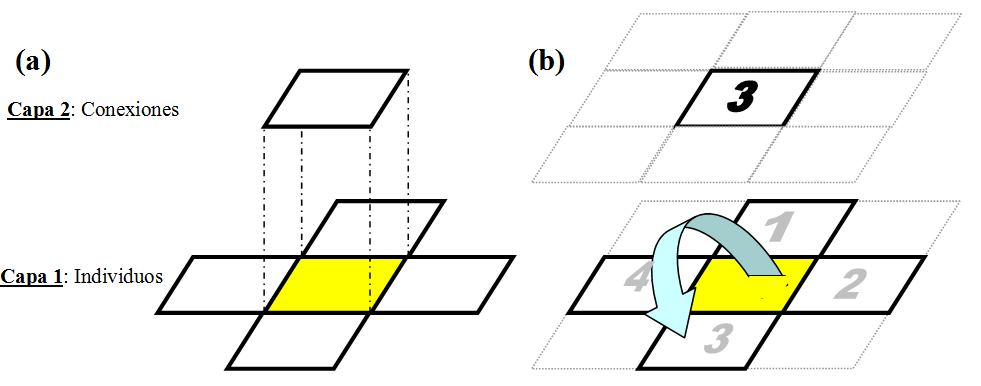
\includegraphics[scale=0.5]{imagenes/modelo_pina.png}
\caption{Vecindario de celdas utilizado para definir el comportamiento de cada agente}
\label{fig:modelo_pina}
\end{figure}

Para extender este vecindario mediante los shock de influencia, definimos modelos atómicos DEVS\cite{DEVS} externos al espacio celular que denominamos \textbf{shockers}. Estos interactúan con una cantidad fija de agentes de la grilla. En la Figura \ref{fig:modelo_shockers} observamos 3 agentes shockers interactuando con 12 celdas cada uno. Esta idea de que los atómicos interactúan con un subconjunto de la población de celdas nos permite generar esta influencia de manera dinámica. Decidimos implementar varios shockers mejorando la performance de ejecución al limitar la cantidad de puertos de salida que estos tienen. La alternativa era tener un solo modelo atómico conectado con todas las celdas de la grilla.  Con esta decisión de diseño es posible variar el tipo de influencia que genera en torno a los grupos con los que interactúa. Por ejemplo con qué periodicidad inyecta un shock, si el shock promueve la indecisión o el extremismo hacia alguno o ambos partidos.

El comportamiento de los shockers está definido de la siguiente manera.

\begin{itemize}
\item Estos atómicos no mantienen un estado.
\item Los puertos de salida están conectados con un subconjunto de las celdas y esta interconexión no varía a lo largo del tiempo. Esta primer interconexión es elegida con distribución equiprobable.
\item En cada instante de tiempo en el cual se produce un shock, para cada shocker se selecciona con probabilidad uniforme un subconjunto de puertos de salida (dentro de sus celdas dominadas) y a estas se les envía una señal.
\item La periodicidad con la cual se realiza un shock forma parte de los parámetros del modelo y está definida en relación con el Tau definido para la interacción de los agentes.
\end{itemize}

\begin{figure}[!h]
\centering
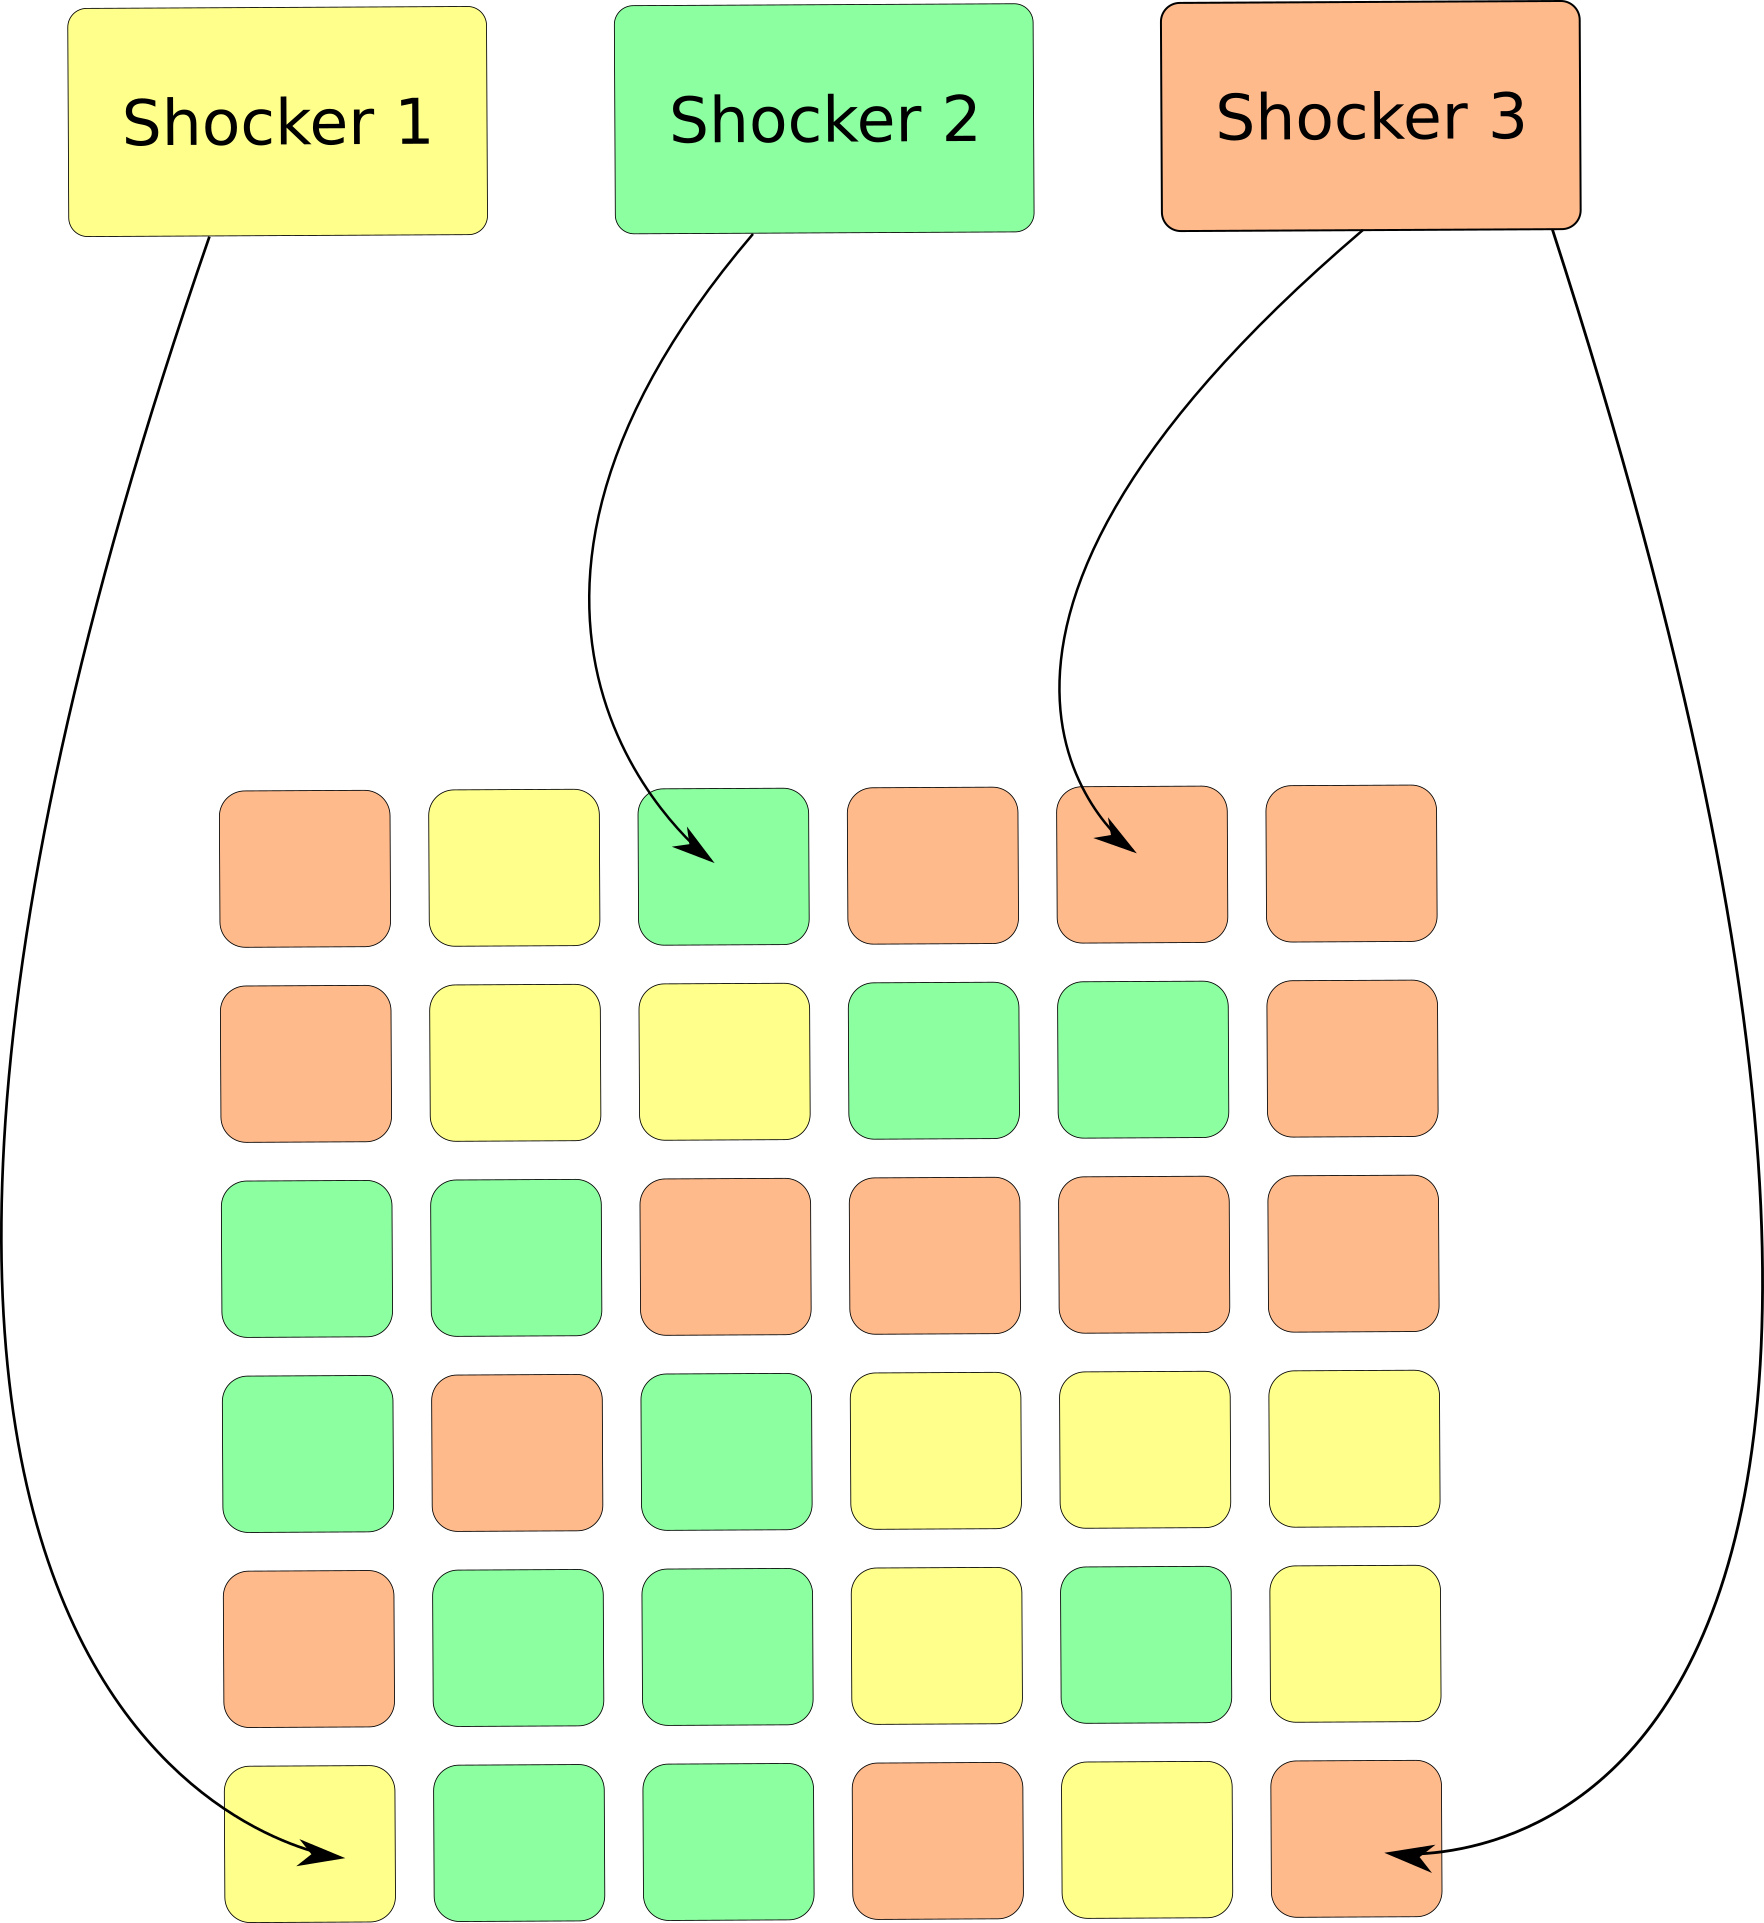
\includegraphics[scale=0.5]{imagenes/agentes_celdas_modelo.png}
\caption{Esquema que muestra el impacto de los shockers sobre el espacio celular}
\label{fig:modelo_shockers}
\end{figure}
